\documentclass[conf]{new-aiaa}
%\documentclass[journal]{new-aiaa} for journal papers
\usepackage[utf8]{inputenc}

\usepackage{graphicx}
\usepackage{amsmath}
\usepackage[version=4]{mhchem}
\usepackage{siunitx}
\usepackage{longtable,tabularx}
\usepackage{float}
\usepackage{subfigmat}
\usepackage{setspace}
\doublespacing

\floatstyle{boxed}
\restylefloat{figure}

\setlength\LTleft{0pt} 

\title{Vector field  path following and obstacle avoidance singularity mitigation via look-ahead flight envelope}

\author{First A. Author\footnote{Insert Job Title, Department Name, Address/Mail Stop, and AIAA Member Grade (if any) for first author.} and Second B. Author Jr.\footnote{Insert Job Title, Department Name, Address/Mail Stop, and AIAA Member Grade (if any) for second author.}}
\affil{Business or Academic Affiliation 1, City, State, Zip Code}
\author{Third C. Author\footnote{Insert Job Title, Department Name, Address/Mail Stop, and AIAA Member Grade (if any) for third author.}}


\begin{document}

\maketitle

\begin{abstract}

Unmanned Aerial Vehicles conventionally navigate by following a series of pre-planned waypoints that may have to be re-planned when flying in a dynamic environment or encountering previously unknown obstacles. Waypoints are generally planned off-line and relayed to the UAV, taking up time and autopilot communication resources. Attractive path following and repulsive obstacle avoidance vector fields have been summed together to produce UAV guidance that follows pre-planned paths and avoids obstacles without the need to re-plan. Summing attractive and repulsive vector fields may produce small regions of null guidance, called singularities, which could potentially lead to trap situations. An investigation into singularity mitigation by vector field weight parameterization is presented. 

% Vector field path following and obstacle avoidance guidance has been used for following a pre-planned path and avoiding obstacles without the need to re-plan the path. 
%
%Re-planning waypoints could be avoided by implementing a path following and obstacle avoidance vector field guidance.
%
%Unmanned Aerial Vehicles (UAVs) conventionally navigate by following a series of pre-planned waypoints generated off-line, which are initially obstacle free, may be to be re-planned when encountering previously unknown obstacles. Re-planning waypoints could be avoided by implementing a path following and obstacle avoidance vector field guidance. Convergent vector fields attract a UAV to follow a path while repulsive vector fields push the UAV away from no-fly zones. Combining attractive and repulsive fields may cause small regions of null guidance, called singularities, which may be avoided by tuning vector field parameters. 
\end{abstract}
%Unmanned Aerial Vehicles (UAVs) conventionally navigate a series of off-line generated and initially obstacle free waypoints that may have to be re-planned when encountering a previously unknown obstacle. Re-planning waypoints could be avoided by implementing a path following and obstacle avoidance vector field guidance. Guidance to converge and follow a pre-planned path is produced by an attractive vector field while obstacles are represented by a repulsive vector field. Summing together attractive goal and repulsive obstacle fields produce a guidance for tracking a pre-planned path while avoiding unplanned obstacles. Small regions of null guidance, called singularities, may be produced when summing attractive and repulsive fields together. 





 

%\textbf{Motivation}
%\begin{itemize}
%	\item Conventional waypoint guidance relies on a pre-planned, flyable, and obstacle free path 
%	\item Obstacles unaccounted for during planning may require a re-plan which may require communication with a ground station
%\end{itemize}
%
%
%\textbf{Background}
%\begin{itemize}
%	\item Vector field guidance for path following has been shown to be both robust in the presence of external disturbances and produce low cross track error flight
%	\item Obstacles can be represented as repulsive fields and summed with attractive fields to produce an obstacle avoidance guidance
%	\item  Summing vector field guidance my produce singularities, resulting in no guidance
%	\item Repulsive fields currently provide no additional information on how to go around obstacle
%\end{itemize}
%
%
%\textbf{Contribution}
%\begin{itemize}
%	\item Method for compensating for singularities that may be experienced (Lookahead or fast detection)
%\end{itemize}




\section{Nomenclature}

{\renewcommand\arraystretch{1.0}
\noindent\begin{longtable*}{@{}l @{\quad=\quad} l@{}}
$UAV$  & Unmanned Aerial Vehicle \\
$VF$   & Vector Field \\
$VFF$  & Virtual Force Field \\
$LVF$  & Lyapunov Vector Field \\
$GVF$  & Goncalves Vector Field \\
\end{longtable*}}

\section{Introduction}
Unmanned Aerial Vehicles are pilotless aircraft used by military, police, and civilian communities for tasks such as reconnaissance, damage assessment, natural disaster surveying, and target tracking \cite{ariyur_autonomous_2008,teuliere_chasing_2011}. Tasks can be performed by a single UAV or with a team of other air, ground, or marine vehicles \cite{oh_coordinated_2013,hyondong_oh_coordinated_2015,ulun_coordinated_2013}. Autonomous vehicle missions are typically accomplished by navigating a series of waypoints \cite{ariyur_autonomous_2008} or path following \cite{oliveira_moving_2016}. Waypoints are conventionally generated off-line at a ground station and relayed over radio to the UAVs autopilot. Obstacles such as buildings, terrain, and other vehicles can be avoided by planning waypoints around obstacles. The on-board guidance directs the UAV towards the current active waypoint, once the UAV has reached a pre-defined distance from the waypoint the UAV is directed to the next waypoint. An example of a UAV following waypoint guidance while avoiding an obstacle is shown in Figure \ref{fig:simplewaypointsWithUAVPath}


\begin{figure}[H]
	\centering
	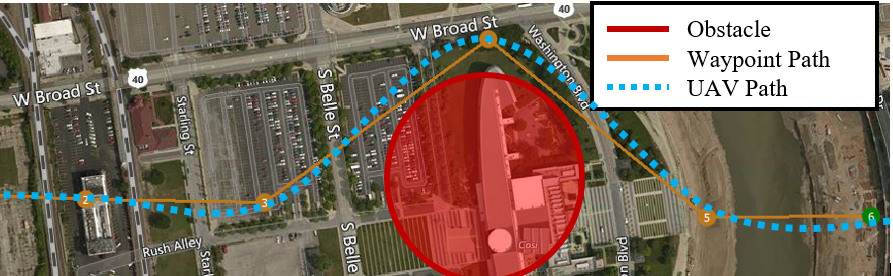
\includegraphics[width=1\linewidth]{Figures/simpleWaypointsWithUAVPath}
	\caption{UAV path from waypoint guidance}
	\label{fig:simplewaypointsWithUAVPath}
\end{figure}


During waypoint navigation the UAV may encounter obstacles or environmental changes that would require a new set of obstacle free waypoints to be generated. For highly uncertain or dynamic environments, there may have to be frequent updates which increases the communication overhead of the autopilot since paths may be updated and communicated from the ground. Additionally, if communication is delayed or lost, waypoints may not be updated rapidly enough and the UAV may fail to avoid the obstacles if the autopilot is following outdated waypoints that violate an obstacle. Real time obstacle avoidance without the need to replan may be found in the use of potential and vector fields, which operate on the principle of artificial attractive and repulsive forces to guide a robotic system. 


\subsection{Potential Field}
Obstacle free paths in static and dynamic environments have been generated with the potential field method, which models a robot's workspace as a gradient of artificial attractive and repulsive forces \cite{khatib_real-time_1986}. Potential field combines path planning, trajectory planning, and control into a single system \cite{rimon_exact_1992}. Paths can be generated by placing a point mass at an initially high potential and allowing it to descend a gradient until the point reaches the goal, located at a global minimum potential. Obstacles provide a limited repulsive force, pushing the mass away from the obstacle. 


A histogram based potential field method can be found in \cite{borenstein_real-time_1990,borenstein_vector_1991,koren_potential_1991} which allowed for real time goal seeking with obstacle avoidance. Sensors on-board a ground robot located at $(x_0,y_0)$ detect obstacles within a pre-defined window containing a fixed number of cells. Cells containing an obstacle provide a repulsive force $\overrightarrow{F_{i,j}}$ opposite in direction to the line-of-sight from vehicle to cell location $(x_i,y_j)$, where $(i,j$) represents the cell index, $F_{cr}$ is a constant repulsive force, $W$ the vehicle's width, $C_{i,j}$ a cell's certainty, and $d_{i,j}$ the distance to the center of the cell with respect to robots center.

\begin{equation}\label{eq:vffRepulse}
\overrightarrow{F_{i,j}} = \frac{F_{cr}W^nC_{i,j}}{d^n_{i,j}} \bigg( \frac{x_i-x_0}{d_{i,j}}\hat{x} + \frac{y_i-y_0}{d_{i,j}}\hat{y}\bigg)
\end{equation}

The total repulsive force exerted on the robot is determined by summing the active cells, shown in Equation \ref{eq:vffRepulseSum}


\begin{equation}\label{eq:vffRepulseSum}
\overrightarrow{F_r} = \sum_{i,j}\overrightarrow{F_{i,j}}
\end{equation}

The robot is attracted to the goal by force $\overrightarrow{F_t}$ with constant magnitude $F_{ct}$ and along the LOS from robot center to goal, located at $(x_t,y_t)$ and a distance $d_t$, shown in Equation \ref{eq:vffGoal}

\begin{equation}\label{eq:vffGoal}
\overrightarrow{F_t} = F_{ct} \bigg( \frac{x_t-x_0}{d_{t}}\hat{x} + \frac{y_t-y_0}{d_{t}}\hat{y}\bigg)
\end{equation}

Summing together attractive and repulsive forces produce a vector that can be used for heading guidance, shown in Equation \ref{eq:vffHeading}.

\begin{equation}\label{eq:vffHeading}
\overrightarrow{R} = \overrightarrow{F_r} + \overrightarrow{F_t}
\end{equation}

 Major drawbacks to potential field were identified in \cite{koren_potential_1991} consisting of local minimum and oscillations in corridors. The local minimum problem occurs when closely spaced obstacle's potential combine to produce a well on the descent gradient where a pre-mature stable point is found. Proposed solutions to local minimum include object clustering and virtual waypoint method \cite{liu_virtual-waypoint_2016}, virtual escaping route \cite{kim_escaping_2009}, and use of navigation functions \cite{goerzen_survey_2010}. Oscillations in potential field were studied in \cite{lei_tang_novel_2010} and \cite{li_efficient_2012}.

In addition to local minimum and oscillations, potential field converges to a singular point which is not possible for fixed wing aircraft since it must maintain a minimum forward velocity to remain airborne. Similar to conventional waypoint guidance, the active goal point would change as a function of proximity. Simulating a UAV using VFF as guidance for a Dubins vehicle was performed and is shown in Figure \ref{fig:vffsimulated}, where a single obstacle cell located at the origin. The UAV initially travels directly toward the goal located at $(50,0)$ until the obstacle is encountered, at which point a repulsive force is applied. The UAV avoids the obstacle, however significantly deviates and fails to get back on the path between waypoints. For certain applications it may be benefitial to follow explicit paths for tasks such as data collection on a roadway or searching a tree line.


\begin{figure}[H]
	\centering
	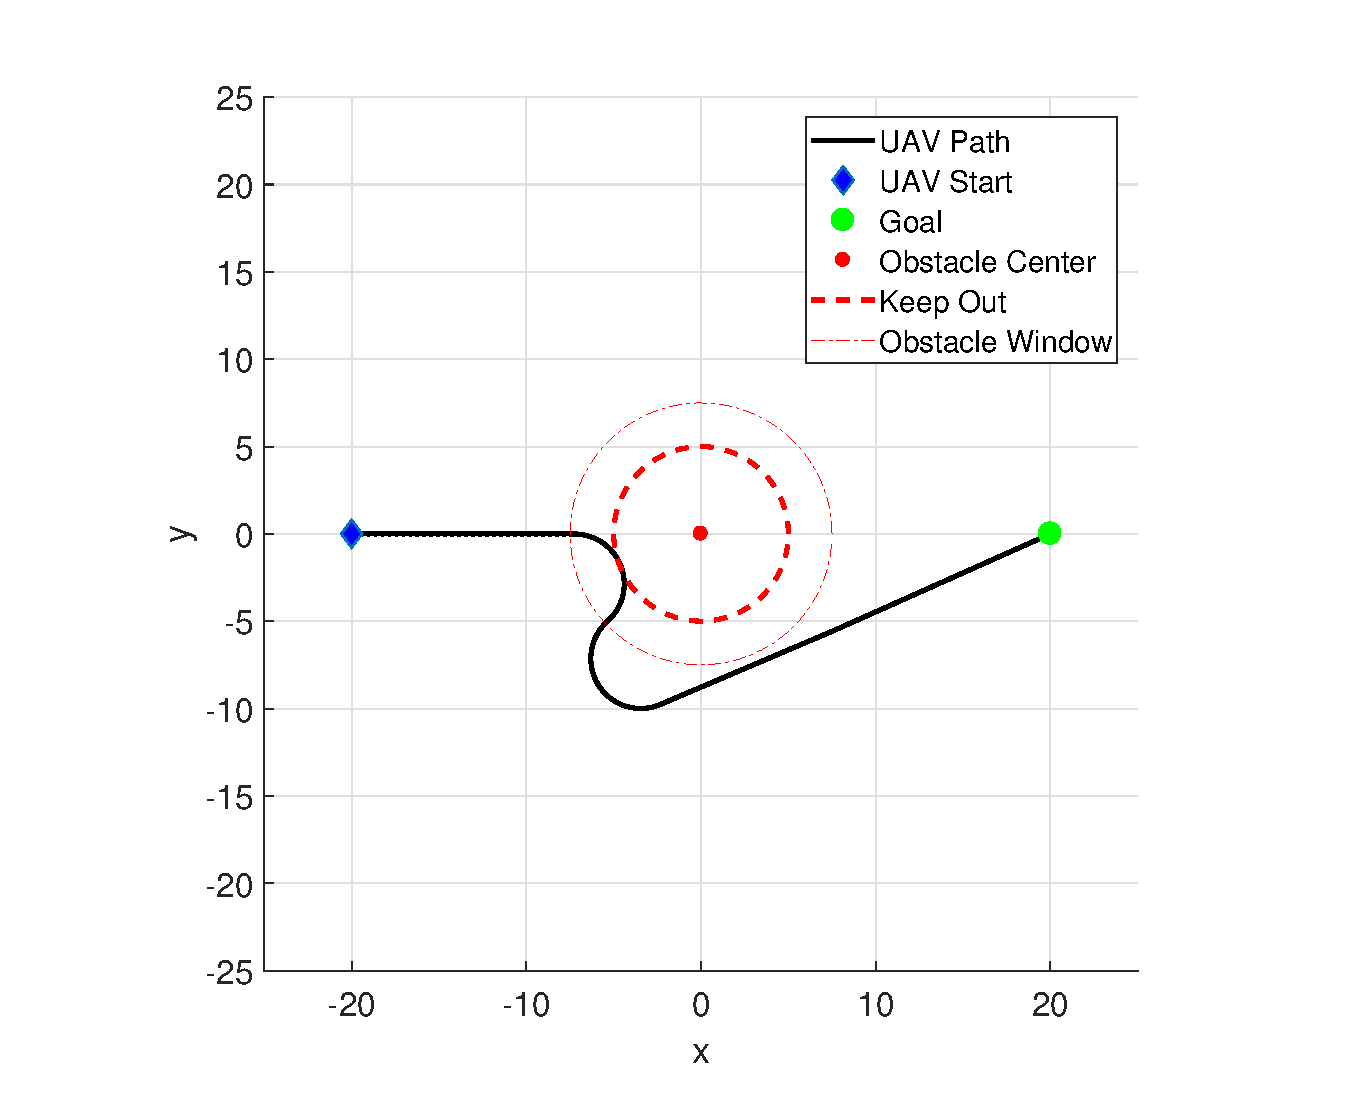
\includegraphics[width=0.7\linewidth]{Figures/vffSimulated}
	\caption{Dubins vehicle encountering an obstacle while navigating to a waypoint}
	\label{fig:vffsimulated}
\end{figure} 



% The potential field method converges to a singular point which is not possible for fixed wing aircraft. Similar to conventional waypoint guidance, the active goal point would change as a function of proximity, however for certain UAV applications such as following a curved ground track or surveying it may be beneficial to follow an explicit path. \\




%A robot at an initially high potential transitions down the gradient to a lower potential. Obstacles are represented by a high potential that act as repulsive forces.
%
%which operates on the principle of attractive and repulsive forces \cite{khatib_real-time_1986}. A robot at an initially high potential is pulled towards a goal located at a globally minimum potential while being repelled by obstacles in close proximity by repulsive forces.

 


%For highly uncertain or dynamic environments, there may have to be frequent updates which may not be possible if communication with the ground station is lost and may not
%
%
%During waypoint navigation the UAV may encounter an obstacle unknown during planning or experience a change in the environment which may require a new obstacle free series of waypoints be generated. A highly uncertain or dynamic environment would require frequent waypoint re-planning which may be difficult or impossible if communication with the ground station is lost. \\


 
%--- Potential Field Methods ----
%Potential field combines path planning, trajectory planning, and control into a single process \cite{rimon_exact_1992}  and is based on the principle of artificial attractive and repulsive forces \cite{khatib_real-time_1986}. 
%
%A robot at an initially high potential is pulled towards a goal located at a globally minimum potential while being repelled by obstacles in close proximity by repulsive forces.
%
% Major drawbacks to potential field were pointed out in \cite{koren_potential_1991} consisting of local minimum and oscillations in corridors. The local minimum problem occurs when closely spaced obstacle's potential combine to produce a well on the descent gradient where a pre-mature stable point is found. Proposed solutions to local minimum include object clustering and virtual waypoint method \cite{liu_virtual-waypoint_2016}, virtual escaping route \cite{kim_escaping_2009}, and use of navigation functions \cite{goerzen_survey_2010}. Oscillations in potential field were studied in \cite{lei_tang_novel_2010}, and \cite{li_efficient_2012}. \\

%The potential field method converges to a singular point which is not possible for fixed wing aircraft. Similar to conventional waypoint guidance, the active goal point would change as a function of proximity, however for certain UAV applications such as following a curved ground track or surveying it may be beneficial to follow an explicit path. \\
	

Following an explicit path to collect data or follow a ground target can be accomplished with vector fields, which produce a heading guidance that asymptotically converges and circulates a path. A comparison between vector field and waypoint guidance techniques was presented in \cite{sujit_unmanned_2014} where each method was evaluated based on its complexity, robustness, and accuracy. The vector field model produced guidance that was both robust to external wind disturbances while maintaining a low cross track error. The two most prominent methods for generating vector fields in literature consist of the Lyapunov \cite{nelson_cooperative_2005,nelson_vector_2006,nelson_vector_2007,frew_cooperative_2007,miao_orthogonal_2016,griffiths_vector_2006} and Goncalves \cite{goncalves_artificial_2009,goncalves_circulation_2010,goncalves_vector_2010,gerlach_autonomous_2014} method. \\

Lyapunov vector fields for converging and following straight and circular paths were described in \cite{nelson_cooperative_2005}. 


%For converging and following a straight path, a guidance vector $\chi^{d}$ is determined in Equation \ref{eq:lyapunovStraight}, where $\chi^{\infty}$ is the course approach angle, $y$ is the lateral distance to the path, and $k$ is a positive constant that determines the rate of transition between convergence and following. An example of a Lyapunov vector field converging and following a straight line is shown in Figure \ref{fig:vfPrimitives}a.
%
%
%
%% and are defined in Equations \ref{eq:lyapunovStraight} and \ref{eq:lyapunovCirc} respectively.
%
%%------ Nelson VF equations -----
%\begin{equation}\label{eq:lyapunovStraight}
%\chi^d(y) = -\chi^{\infty}\frac{2}{\pi}\tan^{-1}(ky)
%\end{equation}
%
%
%
%For converging and following a circular path, a guidance vector $\chi^{d}$ is determined in Equation \ref{eq:lyapunovCirc}, where $\gamma$ is the UAVs angular position with respect to the circle, $r$ is the paths radius, $d$ is the distance from the circles center, and $k$ is a positive constant that determines the transition behavior. An example of a Lyapunov vector field for converging and following a circular path is shown in Figure \ref{fig:vfPrimitives}b.
%
%\begin{equation}\label{eq:lyapunovCirc}
%\chi^d(d) = \gamma-\frac{\pi}{2}-\tan^{-1} \bigg(k \frac{d-r}{r} \bigg)
%\end{equation}
%
%
%\begin{figure}[H]
%	\begin{subfigmatrix}{2}% number of columns
%		\centering	
%		\subfigure []{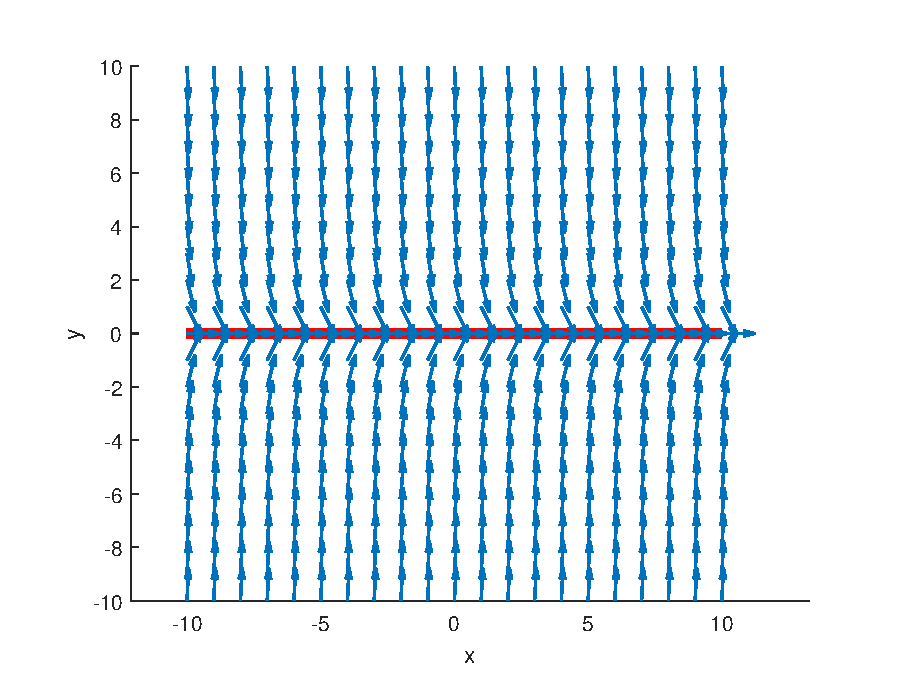
\includegraphics[width=8cm] {Figures/straightLyapunov}}
%		\subfigure []{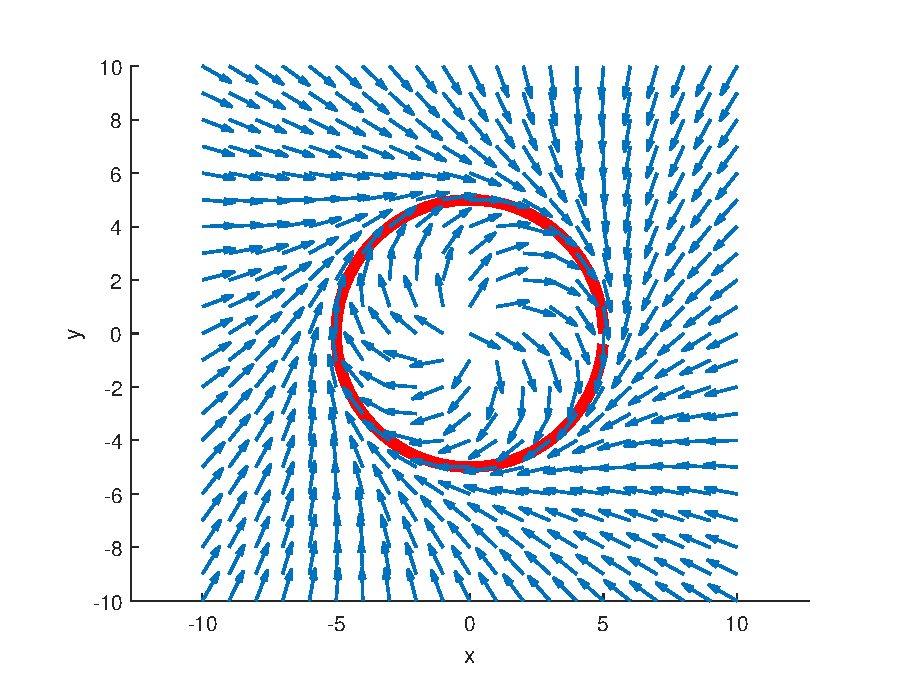
\includegraphics[width=8cm] {Figures/circularLyapunov}}
%		\hspace*{0mm}
%	\end{subfigmatrix}
%	\caption{Lyapunov vector field converging and following a) straight path b) circular path}
%	\label{fig:vfPrimitives}
%%\end{figure}




%A circular Lyapunov vector field can be generated by the methodology described in \cite{frew_cooperative_2007}. Given the Lyapunov function:
%
%
%$y$ lateral distance from path \\
%$\chi$ difference between direction of path and course of UAV \\
%$k$ positive constant that influences the rate of transition \\
%$\chi^{\infty}$  course approach angle at large distance \\
%$\chi^{d}$ is commanded heading \\
%
%$d$ radial distance UAV from center of orbit \\
%$\gamma$ angular position with respect to orbit center \\
%$r$ orbit radius \\
%
%
%
%
%\begin{figure}[H]
%	\begin{subfigmatrix}{2}% number of columns
%		\centering	
%		\subfigure []{\includegraphics[width=7.5cm] {Figures/lineConvcirc}}
%		\subfigure []{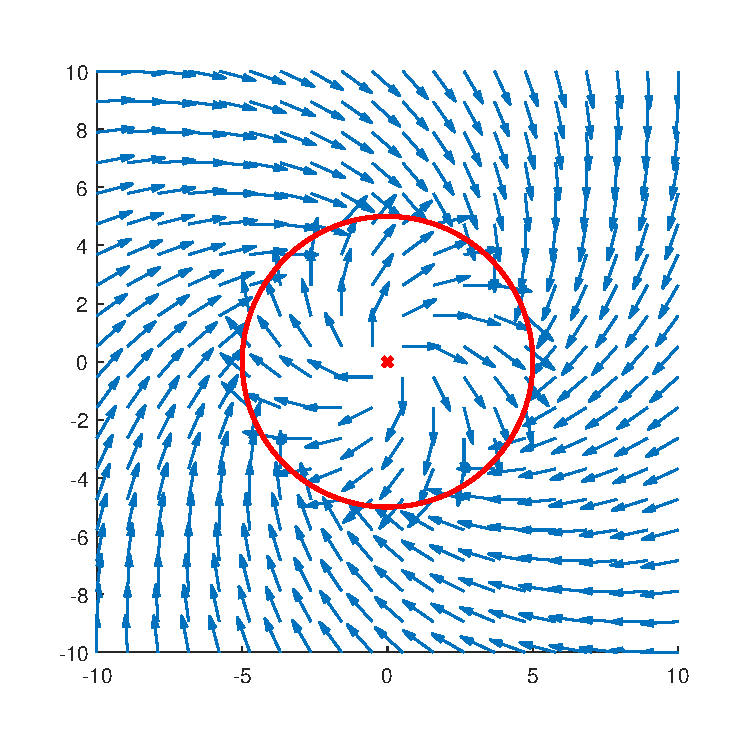
\includegraphics[width=7.5cm] {Figures/circConvCirc}}
%		\hspace*{0mm}
%	\end{subfigmatrix}
%	\caption{Vector field converging and following a) straight path b) circular path}
%	\label{fig:vfPrimitives}
%\end{figure}
%
%
%\begin{equation}\label{eq:lyapunovfunction}
%V(x,y) = (r^2 - r_d^2)^2
%\end{equation}
%where $r$ is given by the equation
%\begin{equation}
%r = \sqrt{x^2+y^2}
%\end{equation}
%and the total time derivative of Equation \ref{eq:lyapunovfunction} is
%\begin{equation}\label{eq:totaltimederivative}
%\dot{V}(x,y) = \nabla{V} \cdotp [\dot{x},\dot{y}]^{T}
%\end{equation}
%Utilizing the following equation to select the desired relative velocity $\dot{x}$ and $\dot{y}$
%\begin{equation}
%\overrightarrow{V}_{Lyapunov}\!=\!\begin{bmatrix} \dot{x_d} \\ \dot{y_d} \end{bmatrix}\!= \alpha\!\left(\dfrac{-v}{r}\right)\!\begin{bmatrix} x \dfrac{r^2-r_d^2}{r^2+r_d^2} + y \dfrac{2 r r_d}{r^2+r_d^2} \\[12pt] y \dfrac{r^2-r_d^2}{r^2+r_d^2} - x \dfrac{2 r r_d}{r^2+r_d^2} \end{bmatrix}
%\end{equation}
%and assuming $\alpha$\,=\,1 and $r$\,=\,1, the final Lyapunov VF equation is generated:
%\begin{equation}\label{eq:lyapunovvf}
%\overrightarrow{V}_{Lyapunov} = \frac{v}{r^2+r_d^2} \begin{bmatrix} - x (r^2-r_d^2) - y (2 r r_d) \\[6pt] - y (r^2-r_d^2) + x (2 r r_d) \end{bmatrix}
%\end{equation}

Straight and circular path vector fields can be selectively activated throughout flight to form more complex paths, shown in \cite{nelson_cooperative_2005,nelson_vector_2006,nelson_vector_2007,jung_unmanned_2016}. Lyapunov vector field for curved path following was presented in \cite{griffiths_vector_2006} which may allow for more complex paths and eliminates the need to switch between vector fields. \\

\subsection{GVF}
The Gonvalves Vector Field (GVF) method produces a similar field, however has several advantages over LVFs. GVF produces an \textit{n}-dimensional vector field that converges and circulates to both static and time varying paths. Additionally, convergence, circulation, and time-varying terms that make up the GVF are decoupled from each other allowing for easy weighting of the total field. GVFs converge and circulate at the intersection, or level set, of $n-1$ dimensional implicit surfaces ($\alpha_i:\mathbb{R}^n\rightarrow\mathbb{R} | i=1,...,n-1$). The integral lines of the field are guaranteed to converge and circulate the level set when two conditions are met: $1)$ the implicit surface functions are positive definite and $2)$ have bounded derivatives. %Consider the space with dimensions in set \textbf{q}:

%The Goncalves Vector Field (GVF) method for producing vector fields has several advantages over the Lyapunov vector field generation methods.


%\begin{equation}
%\mathbf{q} = \begin{bmatrix} x_1, x_2, ..., x_{n}\end{bmatrix}
%\end{equation}

The total vector field $\overrightarrow{V}$ is calculated by:
\begin{equation}\label{eq:GVF}
\overrightarrow{V} = G \nabla V + H \wedge_{i=1}^{n-1}\nabla\alpha_i  - LM(\alpha)^{-1} a(\alpha)
\end{equation}

or in component form:

\begin{equation}\label{simpleGVF}
\overrightarrow{V} = \overrightarrow{V}_{conv} + \overrightarrow{V}_{circ} + \overrightarrow{V}_{tv} 
\end{equation}	

where $\overrightarrow{V}_{conv}$ produces vectors perpendicular to the path, $\overrightarrow{V}_{circ}$ produces vectors parallel to the path, and $\overrightarrow{V}_{tv}$ is a feed-forward term that produces vectors accounting for a time varying path. 

Convergence is calculated by:

\begin{equation}
% Total field with Conv, Circ, and Time
\vec{V}_{conv} = G \nabla V  
\label{convOnly}
\end{equation}

where scalar $G$ is multiplied by the gradient of the definite potential function $V$:

\begin{equation}
V = -\sqrt{{\alpha_1}^2 + {\alpha_2}^2}
\end{equation}



Circulation is calculated by taking the wedge product of the gradients of the surface functions:

\begin{equation}
% Total field with Conv, Circ, and Time
\vec{V}_{circ} =  \wedge_{i=1}^{n-1}\nabla\alpha_i 
\label{circOnly}
\end{equation}

In the case of $(n=3)$ the wedge product simplifies as the cross product:

\begin{equation}
% Total field with Conv, Circ, and Time
\vec{V}_{circ} =  \nabla\alpha_1 \times \nabla\alpha_2 
\label{circOnlySimp}
\end{equation}

The feed-forward time-varying component is calculated by:
\begin{equation}
\label{tv}
\vec{V}_{tv} = M^{-1}a
\end{equation}

where,

\begin{equation}
\label{mMatrix}
M =\begin{bmatrix}
\nabla\alpha_1^T \\
\nabla\alpha_2^T \\
(\nabla\alpha_1 \times \nabla\alpha_2)^T
\end{bmatrix}
\end{equation}

\begin{equation}
\label{aVector}
a =\begin{bmatrix}
\frac{\partial \alpha_1}{\partial t} \quad   \frac{\partial \alpha_2}{\partial t} \quad   0
\end{bmatrix}^T
\end{equation}

Intersecting two flat planes $(\alpha_1 = z,\alpha_2 = x)$ produces a GVF that converges and circulates a straight path, shown in Figure \ref{fig:GVFLine}. 

\begin{figure}[H]
	\begin{subfigmatrix}{2}% number of columns
		\centering	
		\subfigure []{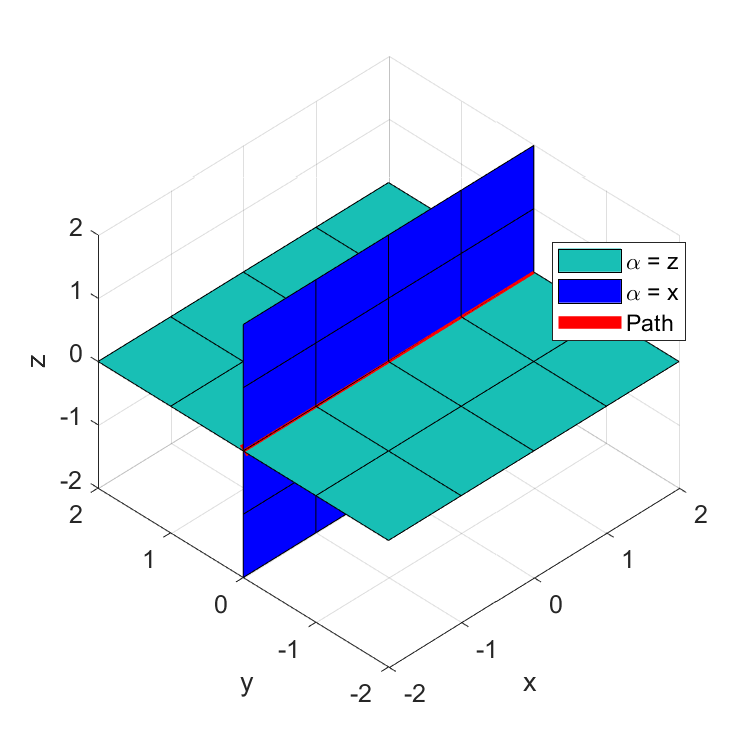
\includegraphics[width=7cm] {Figures/planeIntersection}}
		\subfigure []{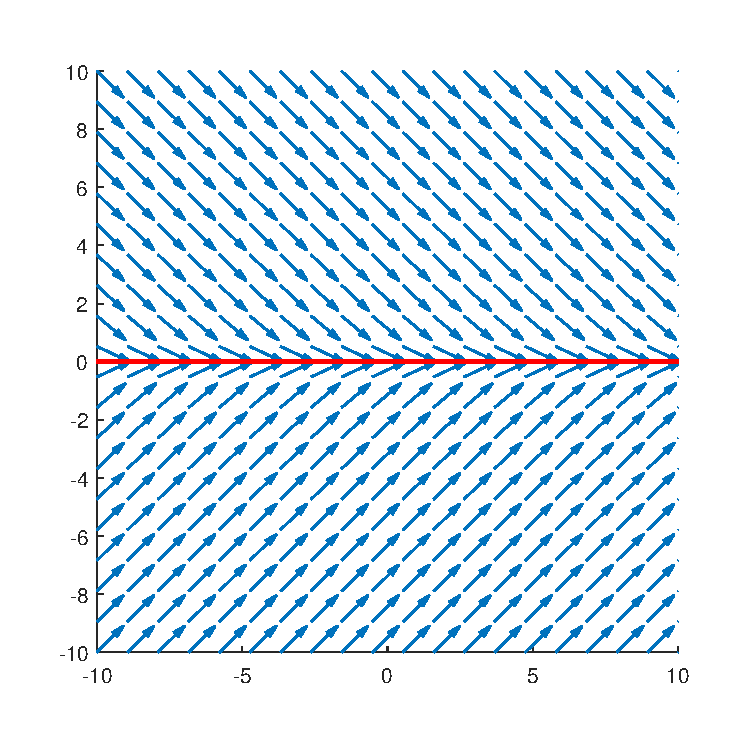
\includegraphics[width=7cm] {Figures/lineConvCirc}}
		\hspace*{0mm}
	\end{subfigmatrix}
	\caption{GVF converging and circulating straight path}
	\label{fig:GVFLine}
\end{figure} 



A GVF for converging and circulating a circular path can be produced by intersecting a plane and a cylinder $(\alpha_1 = z,\alpha_2 = x^2+y^2-r^2)$.
\begin{figure}[H]
	\begin{subfigmatrix}{2}% number of columns
		\centering	
		\subfigure []{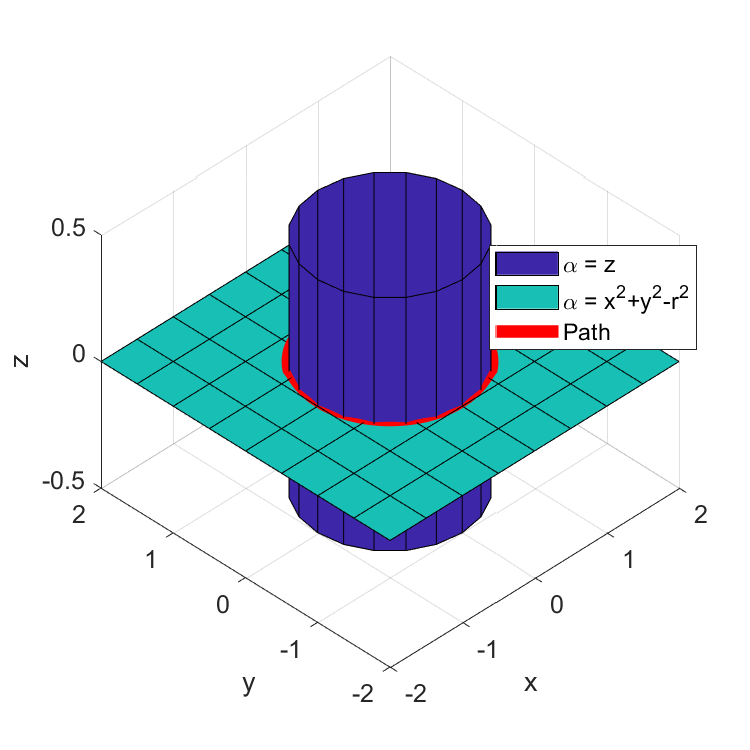
\includegraphics[width=7cm] {Figures/cylinderIntersection}}
		\subfigure []{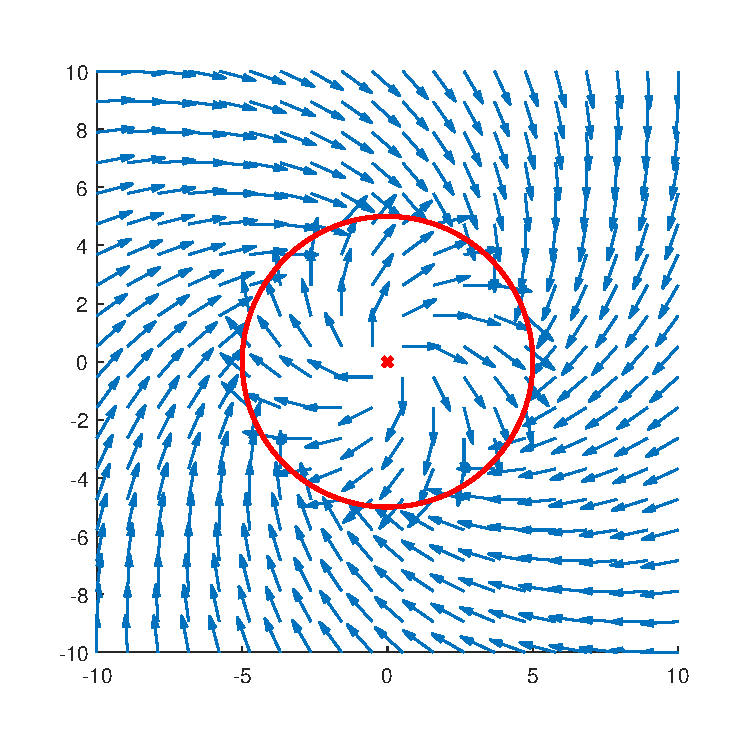
\includegraphics[width=7cm] {Figures/circConvCirc}}
		\hspace*{0mm}
	\end{subfigmatrix}
	\caption{GVF converging and circulating circular path}
	\label{fig:GVFLine}
\end{figure}

%The Goncalves method produces an \textit{n}-dimensional vector field that converges and circulates a static or time-varying path defined by \textit{(n-1)} implicit surfaces ($\alpha_i:\mathbb{R}^n\rightarrow\mathbb{R} | i=1,...,n-1$). The surface functions can represent any shape as long as they satisfy the two conditions that $1)$ they are positive definite and $2)$ have bounded derivatives. Consider the space with dimensions in set \textbf{q}:


GVF was compared against LVP in a standoff tracking scenario in [Wilhelm] where a fixed wing UAV was tasked with with loitering around a moving ground target while avoiding static obstacles.  A circular time-varying attractive vector field was attached to a moving ground target. Static circular repulsive vector fields centered at the obstacles and weighted by hyperbolic tangent decay functions were summed with the attractive circular field to produce a target loitering and obstacle avoidance guidance. The performance of Lyapunov \cite{frew_cooperative_2007} and gradient vector field \cite{goncalves_artificial_2009,goncalves_circulation_2010,goncalves_vector_2010} were compared for their cross track error with respect to the loiter circle. Gradient vector field had favorable performance due to compensation for a time-varying vector field. The gradient vector field technique also has the benefit of decoupled weighting parameters for convergence, circulation, and time-varying terms, allowing for easy modification of field behavior. \\

Decay functions for avoidance fields using GVF were investigated in [Zhu] for obstacles present on a straight path. When summing attractive and repulsive vector fields there is the possibility of guidance singularities, where magnitude and direction are equal and opposite. The presence of singularities were not addressed in [Wilhelm] and [Zhu], mentioned briefly in \cite{nelson_cooperative_2005} and observed in \cite{panagou_motion_2014}. For fixed wing UAVs the lack of guidance may prevent the UAV from avoiding an obstacle, while multi-rotor UAVs may end up in a trap situation. Singularities may be present at any location where a goal field and obstacle field are of equal strength. \\


\subsection{Dubins Vehicle}
Dubin's vehicle's position $\overrightarrow{X}$ at time $t$ is calculated from the integral of the velocity vector $\overrightarrow{U}$. The vehicle has a constant velocity magnitude $u_{uav}$ at a heading $\theta$. The rate at which $\theta$ changes with respect to time is based on limitations of the craft itself. 

\begin{equation}
\label{uavVelocity}
\overrightarrow{U}(t) = u_{uav} \begin{bmatrix}
cos(\theta(t)) \\
sin(\theta(t))
\end{bmatrix}
\end{equation}


\begin{equation}
\label{uavPosition}
\overrightarrow{X}(t) = \overrightarrow{U}dt + \overrightarrow{X}(t-1)
\end{equation}


\begin{equation}
\label{turnRate}
\dot{\theta} \leq 20 deg/s
\end{equation}




\section{methods}
Overview of methods \\
Construction of guidance for desired path \\
Construction of avoidance guidance \\
Path following and obstacle avoidance guidance \\
Singularity detection \\
Selection of vf parameters for optimized obstacle avoidance \\

\subsection{Path Following with GVF}
Path following guidance for a planar UAV at position $(x,y)$ for a time invariant line is achieved by summing together convergence $\overrightarrow{V}_{conv}$ and circulation $\overrightarrow{V}_{circ}$ terms shown in Equation \ref{eq:convAndCircOnly}.

\begin{equation}
\label{eq:convAndCircOnly}
\overrightarrow{V} = \overrightarrow{V}_{conv} + \overrightarrow{V}_{circ} 
\end{equation}

where

\begin{equation}
\label{eq:timeInvariantPath}
 \overrightarrow{V}_{conv} = G \nabla V
\end{equation}

and the potential function V is

\begin{equation}
\label{potentialFunction}
V = -\sqrt{\alpha_1^2+\alpha_2^2}
\end{equation}


where the plane defined by implicit surface function $\alpha_1$ is at angle $\delta$ and plane $\alpha_2$ is at constant height of $Z = 1$ shown in Equations \ref{eq:pathFunction} and \ref{eq:pathFunctionZ} respectively.


\begin{equation}
\label{eq:pathFunction}
\alpha_1 = cos(\delta)x + sin(\delta)y
\end{equation}

\begin{equation}
\label{eq:pathFunctionZ}
\alpha_2 = z
\end{equation}

The gradient $\nabla$ of the potential function $V$ is shown in Equation \ref{eq:potentialFunctionGrad}.

\begin{equation}
\label{eq:potentialFunctionGrad}
\nabla V = -\frac{1}{2(\sqrt{\cos^2(\delta) x^2+2\cos(\delta)\sin(\delta) xy +\sin^2 (\delta) y^2})} \begin{bmatrix}
2x\cos^2(\delta) + 2\cos(\delta)\sin(\delta) y \\
2y\sin^2(\delta) + 2\cos(\delta)\sin(\delta) x \\
2
\end{bmatrix}
\end{equation}

Circulation is calculated by the cross product of the surface function gradients, shown in Equation \ref{eq:circStraightPath} and \ref{eq:circStraightPat2}.


\begin{equation}
\overrightarrow{V}_{circ} =  \nabla \alpha_1 \times \nabla \alpha_2 
\label{eq:circStraightPath}
\end{equation}


\begin{equation}
\label{eq:circStraightPat2}
\overrightarrow{V}_{circ} = \begin{bmatrix}
cos(\theta) \\
sin(\theta) \\
0
\end{bmatrix}
\end{equation}

Guidance for a path at angle $\delta = 0$ and equal parts circulation and convergence weights $G=H=1$ is shown in Figure \ref{fig:straightpath} below.

\begin{figure}[H]
	\centering
	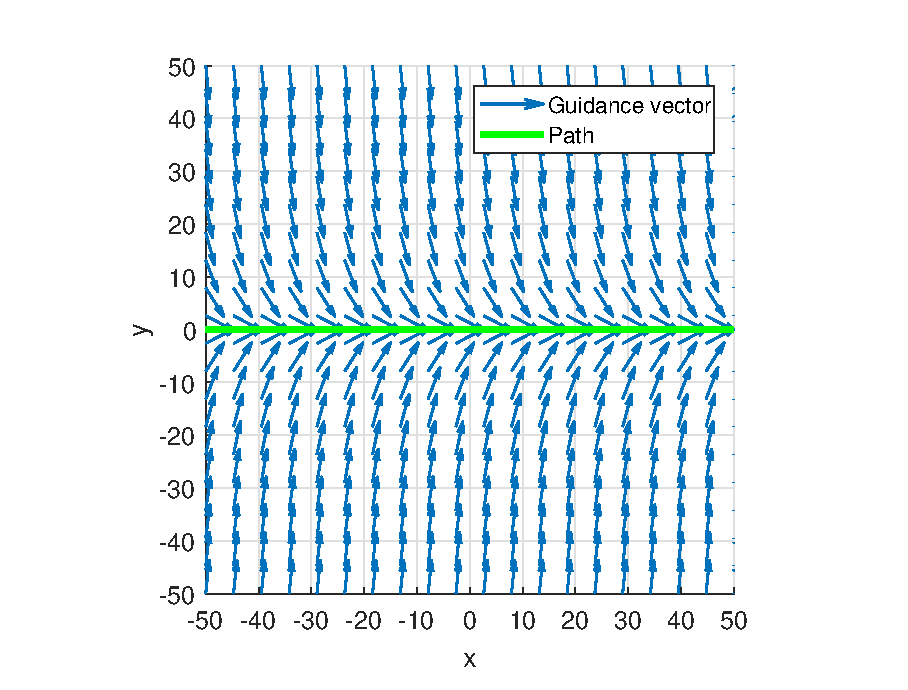
\includegraphics[width=0.7\linewidth]{Figures/methods/straightPath}
	\caption{}
	\label{fig:straightpath}
\end{figure}



\subsection{Avoidance}

Constructing a repulsive vector field for avoidance using the GVF method starts with constructing a vector field that converges and circulates a circular path. A GVF that converges and circulates a circular path is constructed with the implicit functions of a cylinder of radius $r$ centered at $(x_c,y_c)$ and a level plane of constant height $Z$, shown in Equations \ref{eq:alphaCylinder} and \ref{eq:alphaPlane} below.

\begin{equation}\label{eq:alphaCylinder}
\alpha_1 = (x-x_c)^2 + (y-y_c)^2-r^2
\end{equation}

\begin{equation}\label{eq:alphaPlane}
\alpha_2 = z
\end{equation}

Convergence is determined by the gradient of the potential function \ref{eq:potentialFunctionGrad}, which when simplified evaluates to

\begin{equation}
\overrightarrow{V}_{conv} = A\overrightarrow{B}
\end{equation}

where


\begin{equation}
A = \dfrac{-1}{\sqrt{\bar{x}^4+\bar{y}^4+2\bar{x}^2\bar{y}^2-2r^2\bar{x}^2-2r^2\bar{y}^2+r^2+z^2}}
\end{equation}

and

\begin{equation}
\overrightarrow{B} = \begin{bmatrix} 2\bar{x}^3+2\bar{x}\bar{y}^2-2r^2\bar{x} \\ 2\bar{y}^3+2\bar{x}^2\bar{y}-2r^2\bar{y} \\z \end{bmatrix}
\end{equation}.




\begin{equation}
\bar{x} = x - x_c
\end{equation}
\begin{equation}
\bar{y} = y - y_c
\end{equation}

Circulation is calculated from the cross product of each implicit surface functions gradient, which simplifies to

\begin{equation}\label{eq:vcirc_circle}
\overrightarrow{V}_{circ} =  \begin{bmatrix}  2(y-y_c) \\[6pt] -2(x-x_c) \\[6pt] 0\end{bmatrix}
\end{equation}

Guidance for avoiding a circular path with a large radius can be produced by setting the convergence weight $G=-1$ and circulation weight $H=0$, shown in Figure \ref{fig:largerepulsive}. Note that the vectors are normalized prior to applying decay to ensure the vector field strength is bounded.

\begin{figure}[H]
	\centering
	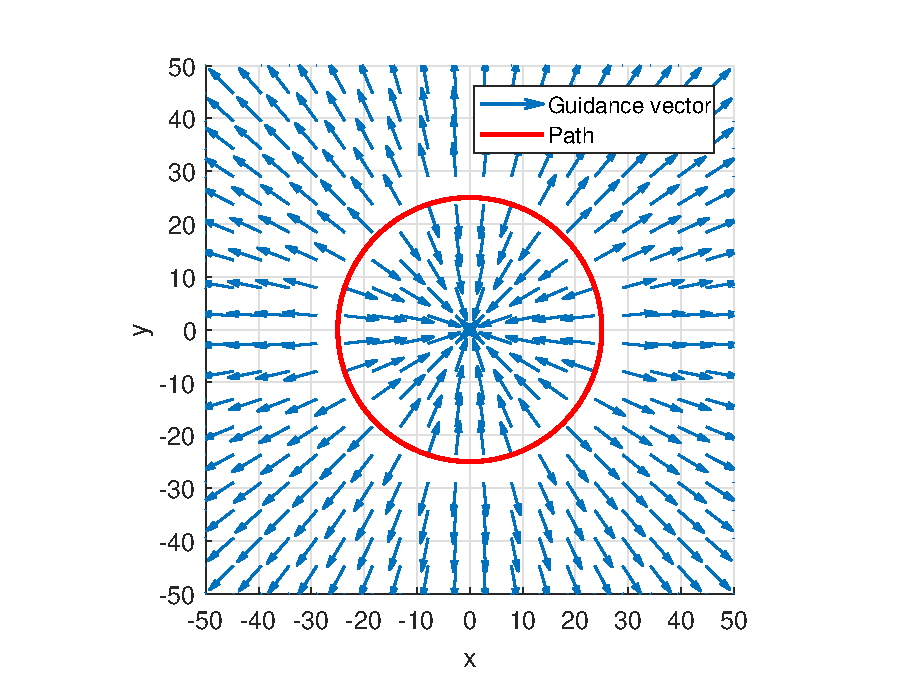
\includegraphics[width=0.7\linewidth]{Figures/methods/largeRepulsive}
	\caption{}
	\label{fig:largerepulsive}
\end{figure}

Note that inside of the path, vectors point towards the center of the circle which may produce a trap situation if the UAV ends up inside the radius. To prevent a trap situation inside of the circular path, the radius of the path can be reduced, as shown in Figure \ref{fig:normalizedrepulsive} where $r=0.01$.


\begin{figure}[H]
	\centering
	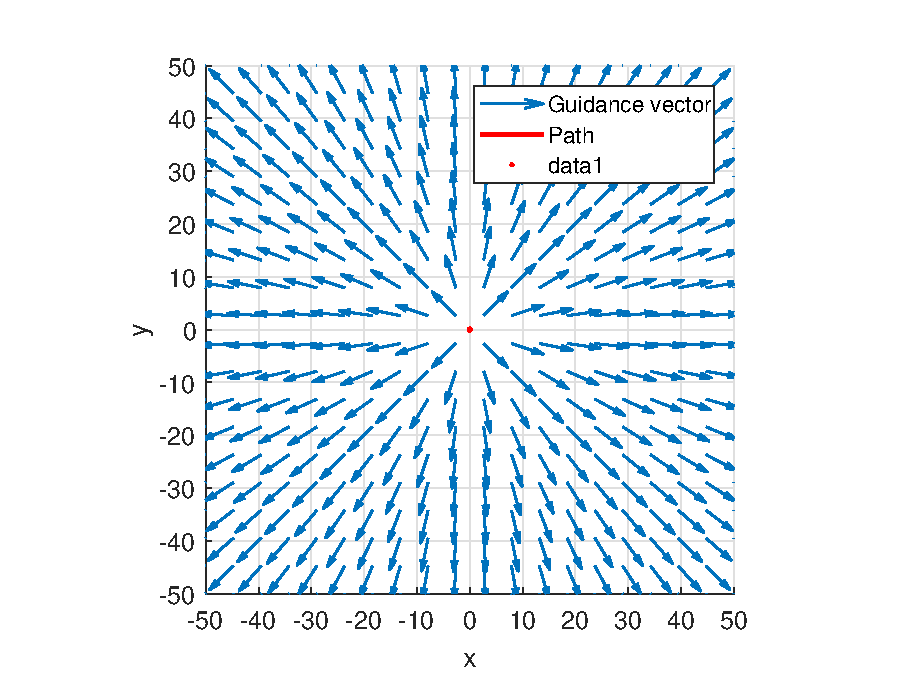
\includegraphics[width=0.7\linewidth]{Figures/methods/normalizedRepulsive}
	\caption{}
	\label{fig:normalizedrepulsive}
\end{figure}

To limit the influence of the repulsive field to a radius $R$, a decay function is applied prior to summing with the path following guidance. The decay strength $P$ is determined in \ref{eq:decay}, where $d$ is the euclidean distance, or range, between the UAV and the center of the obstacle, shown in Equation \ref{eq:range}. At a distance $d>R$ the decay strength $P$ is effectively zero, having virtual no influence on the total guidance. At a distance $d\leq R$, the field strength is bounded between $[0,2]$.


\begin{equation}
\label{eq:decay}
P = -\tanh \bigg( \frac{2\pi d}{R}-\pi\bigg)+1
\end{equation}

\begin{equation}
\label{eq:range}
d = \sqrt{ \bar{x}^2+\bar{y}^2}
\end{equation}

Applying the decay function with a decay edge radius $R = 35$ to the GVF shown in figure \ref{fig:normalizedrepulsive}, results in the field shown in Figure \ref{fig:decayapplied}.


%\begin{figure}[H]
%	\centering
%	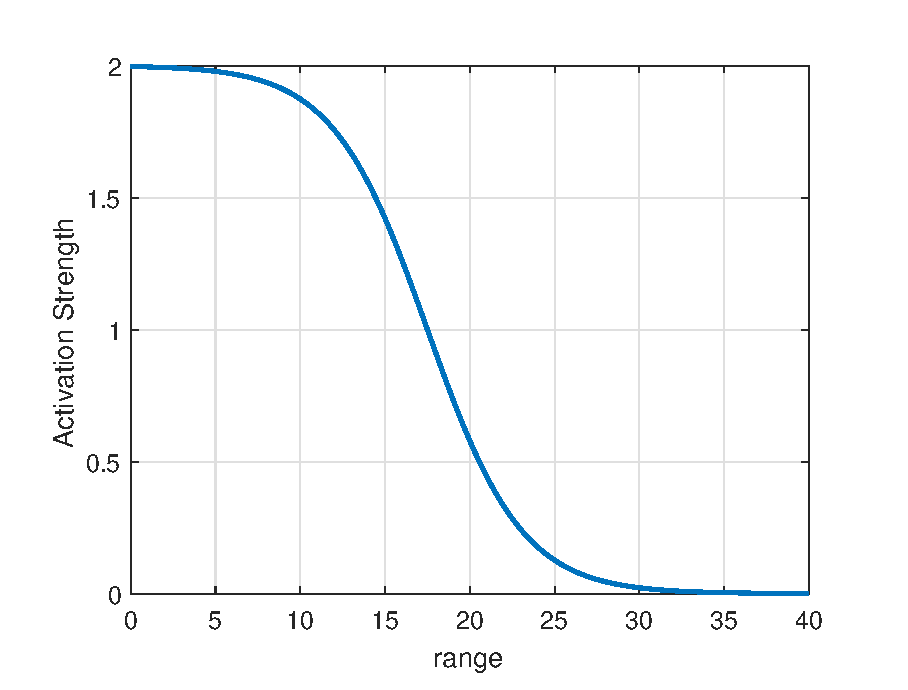
\includegraphics[width=0.7\linewidth]{Figures/methods/tanH}
%	\caption{}
%	\label{fig:tanh}
%\end{figure}



\begin{figure}[H]
	\centering
	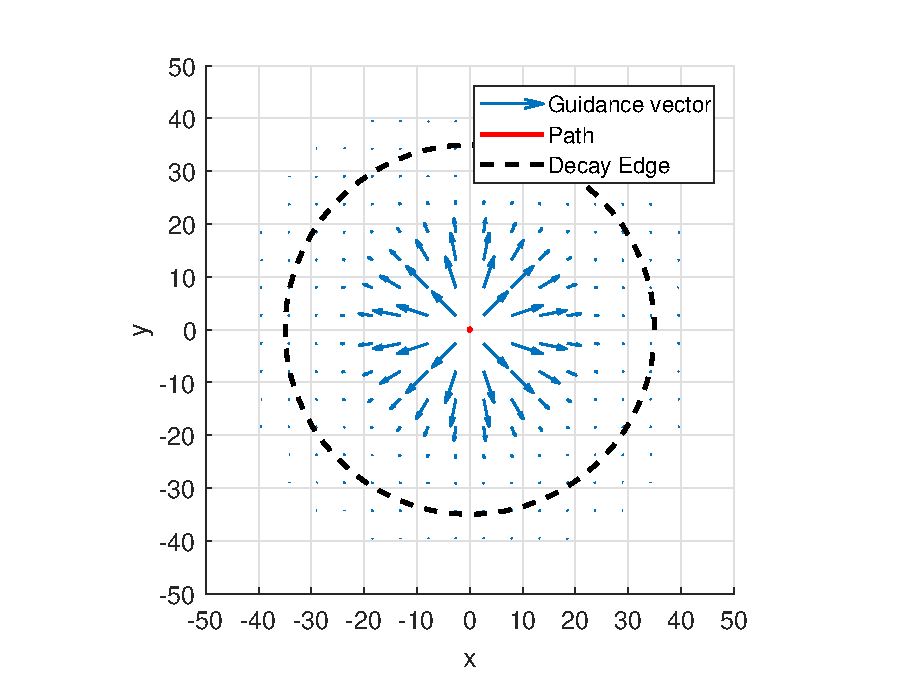
\includegraphics[width=0.7\linewidth]{Figures/methods/decayApplied}
	\caption{}
	\label{fig:decayapplied}
\end{figure}

%\begin{figure}[H]
%	\centering
%	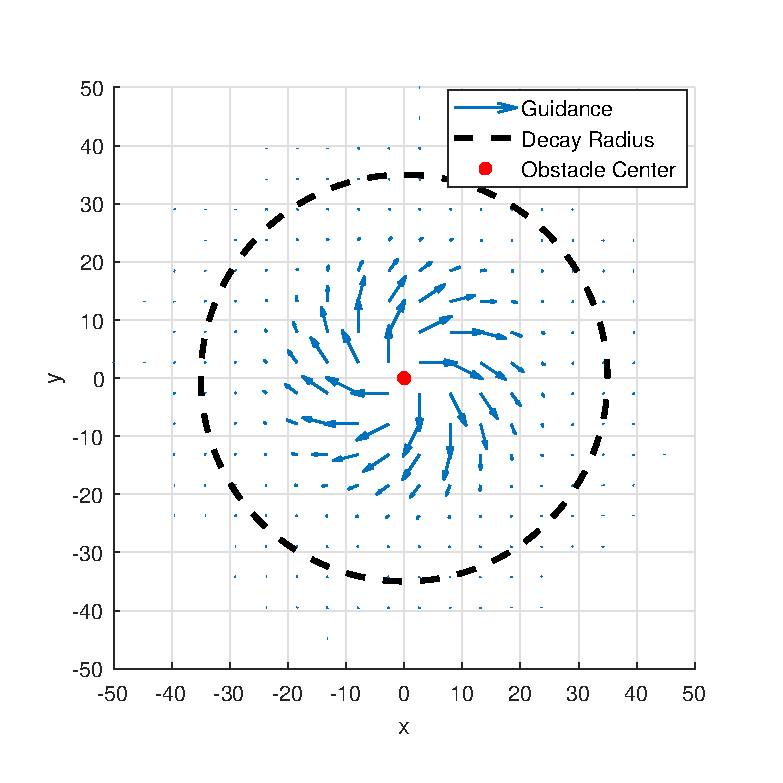
\includegraphics[width=0.7\linewidth]{Figures/methods/decayAppliedCirculation}
%	\caption{}
%	\label{fig:decayappliedcirculation}
%\end{figure}

Summing together the path following field with an obstacle centered on the path results in the guidance $\overrightarrow{V}_G$ shown in Figure \ref{fig:summedquiver}.

\begin{equation}
\label{eq:singularityCondition}
\overrightarrow{V}_g = \overrightarrow{V}_{path} + P\overrightarrow{V}_{obst}
\end{equation}




\begin{figure}[H]
	\centering
	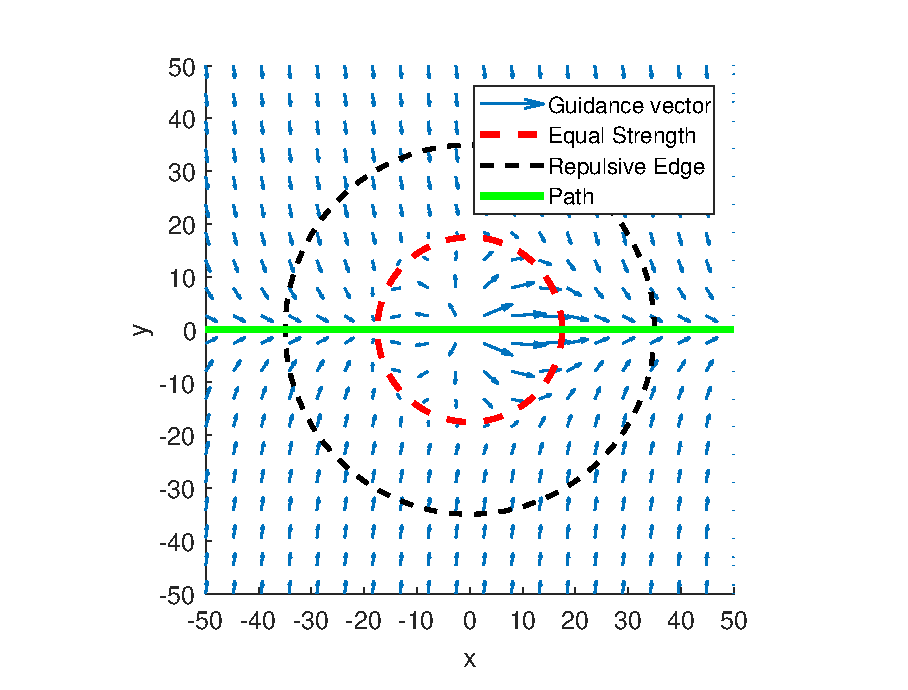
\includegraphics[width=0.7\linewidth]{Figures/methods/summedQuiver}
	\caption{}
	\label{fig:summedquiver}
\end{figure}










\subsection{Singularity Detection}
\begin{equation}
\label{eq:singularityCondition}
||\overrightarrow{V}_g || = 0
\end{equation}

Summing GVFs together may lead to small regions where the vector magnitude is near or equal to zero. Singularities are expected to exist where two summed fields have equal strength. The location of the singularities can be found by determining where the magnitude of the resulting guidance is equal to zero.


Plotting the magnitude of the summed field near the obstacle shows a well that descends into several local minimums called singularities, shown in Figure \ref{fig:summedmagnitudesurf}.


\begin{figure}[H]
	\centering
	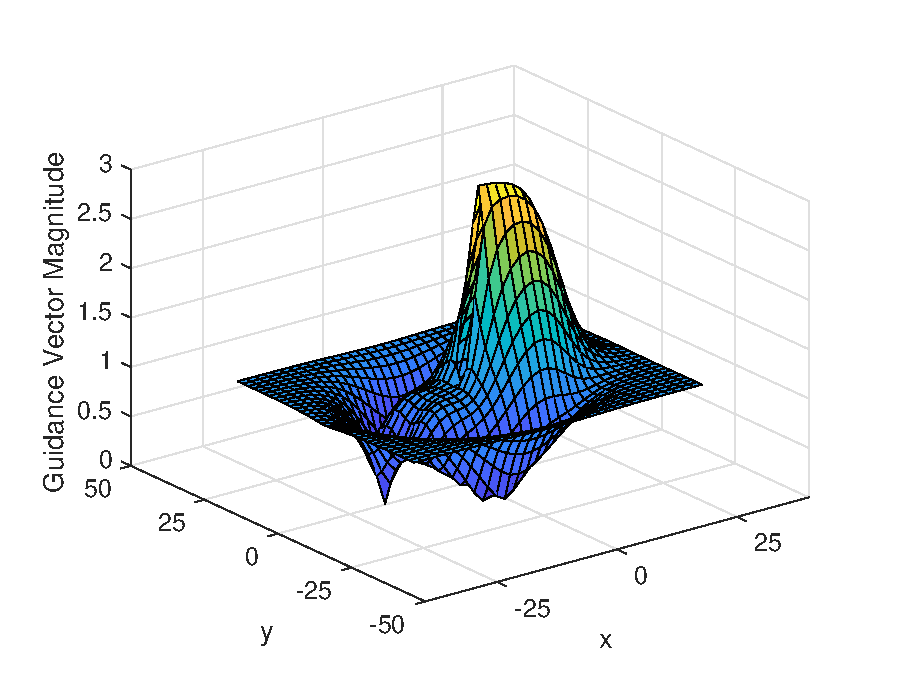
\includegraphics[width=0.7\linewidth]{Figures/methods/summedMagnitudeSurf}
	\caption{}
	\label{fig:summedmagnitudesurf}
\end{figure}

%Before using vector field guidance it is beneficial to know if singularities exist, where they are, and if the UAV will encounter them during flight. Singularities are expected to exist where two summed fields have equal strength. The location of the singularities can be found by determining where the magnitude of the resulting guidance is equal to zero.
 Multiple singularities or near zero guidance regions may exist, so several initial conditions must be evaluated to increase the probability of detection. With the path and obstacle field shown in \ref{fig:summedquiver}, several initial conditions evenly spaced were evaluated both inside and outside of the equal strength circle. Note how only points left of the obstacle were evaluated since this region is where attractive and repulsive vectors oppose each other, therefore it is where singularities are expected. Both inside and outside initial conditions determine the location of the singularities. 

\begin{figure}[H]
	\begin{subfigmatrix}{2}% number of columns
		\centering	
		\subfigure []{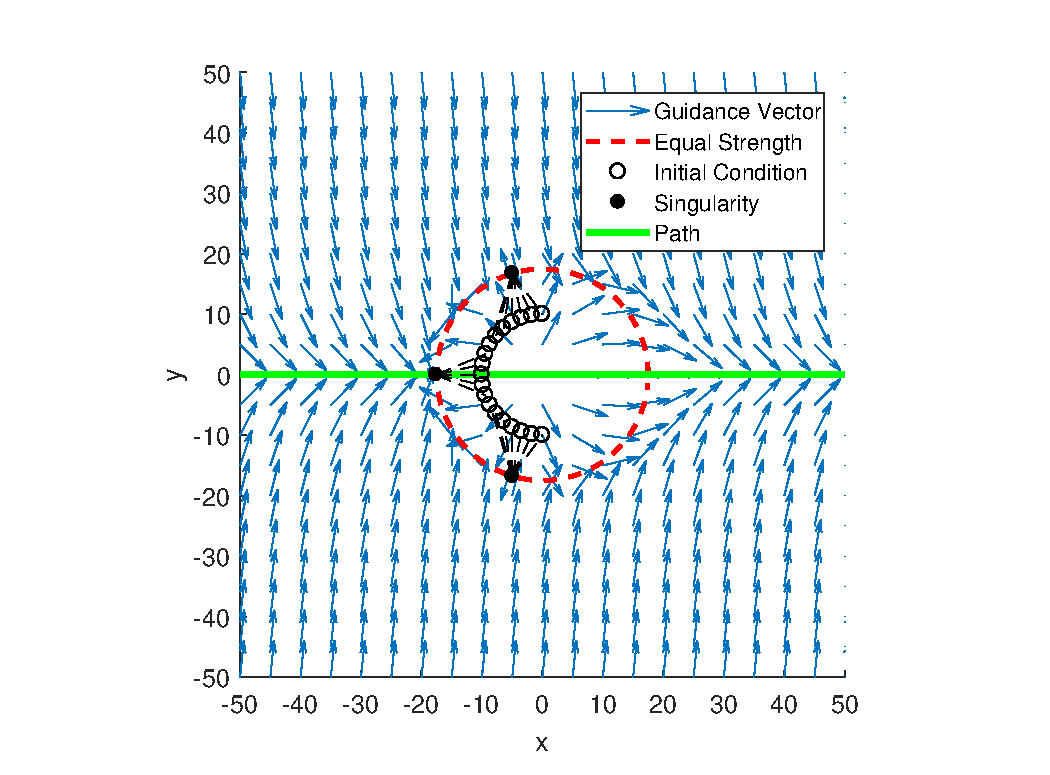
\includegraphics[trim=70 0 70 0,clip,width=8cm] {Figures/methods/noCircSingularityR10}}
		\subfigure []{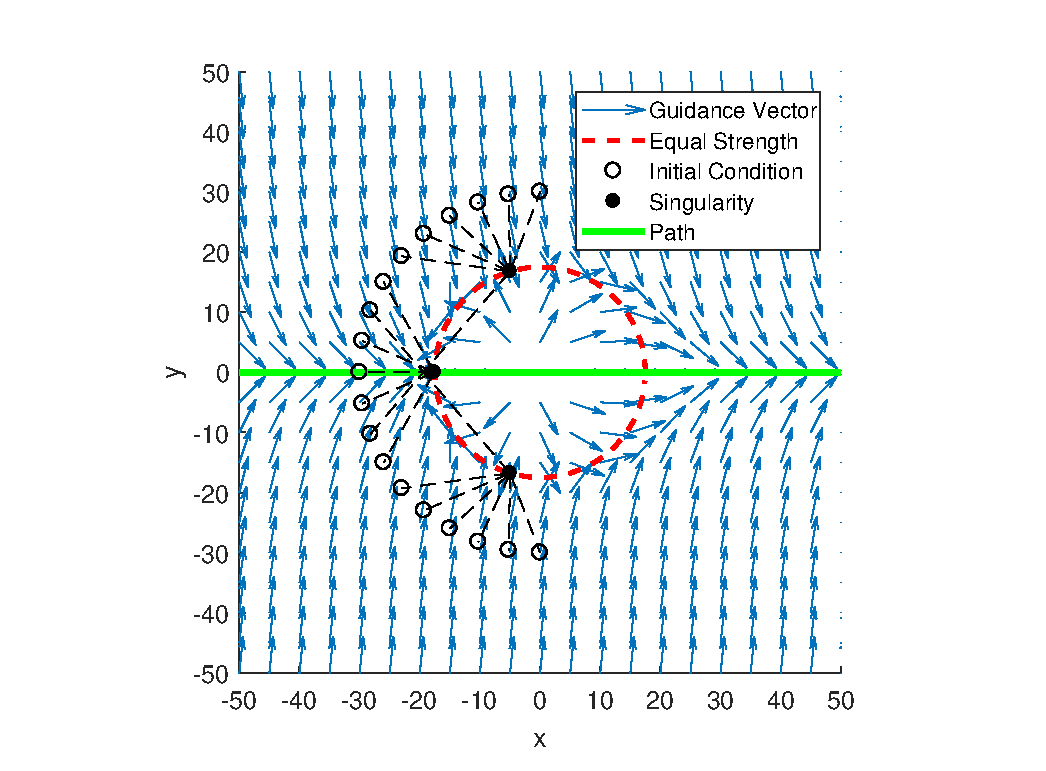
\includegraphics[trim=70 0 70 0,clip,width=8cm] {Figures/methods/noCircSingularityR30}}
		\hspace*{0mm}
	\end{subfigmatrix}
	\caption{GVF converging and circulating circular path}
	\label{fig:noCircSingularityDetection}
\end{figure}










\subsection{Flight Envelope}
Evaluating a large number of initial conditions to improve the probability of finding singularities may be computationally expensive and may also find singularities the UAV may not encounter. Selecting a reduced set of initial conditions and to determine if the singularities exist where the UAV may fly, a flight envelope is determined for some time horizon $t_h$. Consider the UAV depicted in Figure \ref{fig:flightenvelope2} with a turn rate $\dot{\theta}$ and fixed speed $u$. 

\begin{figure}[H]
	\centering
	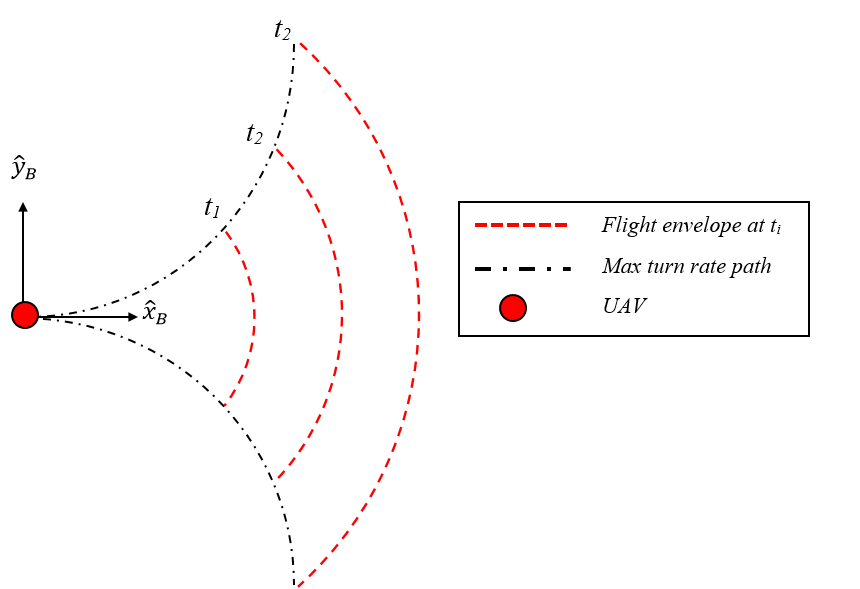
\includegraphics[width=0.7\linewidth]{Figures/methods/flightEnvelope2}
	\caption{}
	\label{fig:flightenvelope2}
\end{figure}

The flight envelope, or positions the UAV, at time $t_i$ with respect to the body frame is calculated in Equations \ref{eq:qx} and \ref{eq:qy}

\begin{equation}
\label{eq:qx}
q_x =  \frac{u}{\dot{\theta}} \sin(t_h \dot{\theta})
\end{equation}

\begin{equation}
\label{eq:qy}
q_y =  \frac{u}{\dot{\theta}} \big(1-\cos(t_h \dot{\theta})\big)
\end{equation}

It is convenient to represent points on the flight envelope in the global inertial frame. The flight envelope points $(q_x,q_y)$ can be expressed in vector form by finding the angle $\phi$ with respect to the body frame $\hat{x}_b$ axis and the vector magnitude $q$ shown in equations \ref{eq:qphi} and \ref{eq:qMag} respectively.




\begin{equation}
\label{eq:qphi}
\phi = \tan^{-1} \bigg( \frac{q_y}{q_x} \bigg)
\end{equation}

\begin{equation}
\label{eq:qMag}
q = \sqrt{q_x^2 +q_y^2}
\end{equation}



\begin{equation}
\label{eq:pos}
\overrightarrow{Q_b} = \begin{bmatrix}
	q\cos\phi \\
	q\sin\phi \\
	0
\end{bmatrix}
\end{equation}

To express the flight envelope in the global inertial frame, the position vector of the UAV $\overrightarrow{P}_0$ and $\theta$ are applied with a rotation matrix $R$, shown in Equations \ref{eq:pos}, \ref{eq:rotation}, and \ref{eq:qGlobal} below. 


\begin{figure}[H]
	\centering
	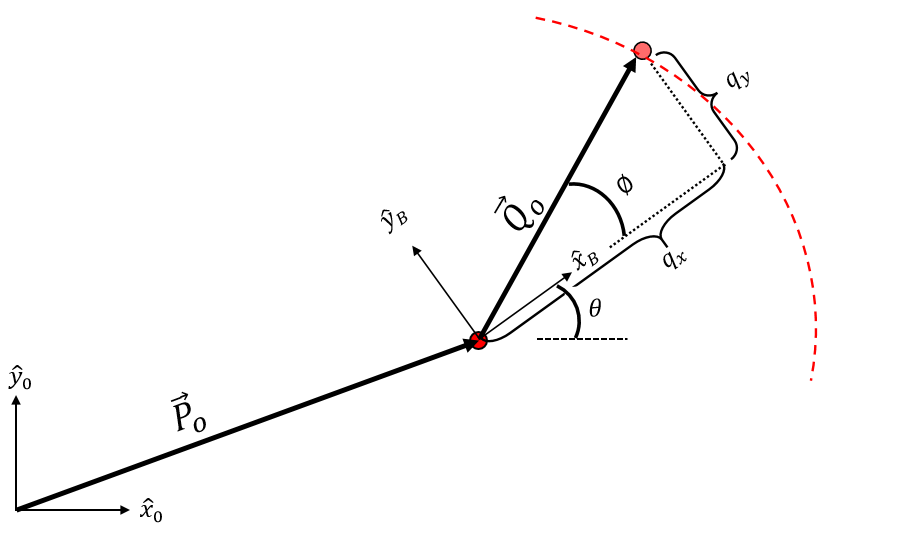
\includegraphics[width=0.7\linewidth]{Figures/methods/flightEnvelope}
	\caption{}
	\label{fig:flightenvelope}
\end{figure}


\begin{equation}
\label{eq:rotation}
\overrightarrow{P}_0 = \begin{bmatrix}
x & y & 0
\end{bmatrix}^T
\end{equation}


\begin{equation}
\label{eq:qGlobal}
   R=\begin{bmatrix}
	\cos(\theta) & -\sin(\theta) & 0 \\
	\sin(\theta) & \cos(\theta) & 0 \\
	0 & 0 & 1 \\
\end{bmatrix}
\end{equation}


\begin{equation}
\label{eq:pos}
\overrightarrow{Q}_0 = \overrightarrow{P_0} + R  \overrightarrow{Q_b}
\end{equation}


Initial conditions placed on the flight envelope will follow the magnitude gradient of the GVF guidance and locate any singularities it may encounter. When a singularity is found to exist inside or near a flight envelope the field can be modified to counteract it. 




\section{Conclusion}



\section*{Appendix}



\section*{Acknowledgments}

\bibliography{bib}

\end{document}
